\subsection{Discussion}
% Mandatory: Create screenshots using Google Earth for each of the scenarios of the collected KML files. The screenshots should include a path that marks the actually walked route. Comment on the results in the report and discuss how GPS errors impacted the results.
% Mandatory: Make a list with the following entries for each scenario: strategy, number of GPS fixes, number of uplink messages, time span, GPS fixes per second, uplink messages per second and comment on them in the report with respect to relevant literature. Discuss what pervasive positioning applications the different strategies are relevant for.
The various methods for reading GPS have various advantages and disadvangtages. The periodic reporting strategy sends a big amount of locations as seen in figure-\ref{locationsreadandsent}, this have the advantage of getting a huge precision of the user and being able to track the movement in a detailed way. This also overcomes the issue with cutting corners off that the distance based algorithms have. The downside of this is that the amount of GPS readings and sending data to the server would also increase the battery use a lot. Thus this will be most suitable in cases where a high precision is needed.

\begin{figure}[h]
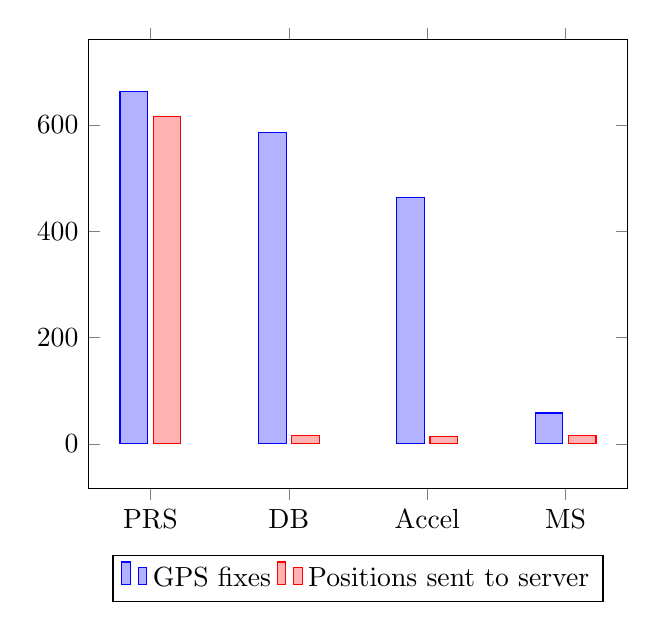
\begin{tikzpicture}
\begin{axis}
	[ybar,
	enlargelimits=0.15,
	legend style={at={(0.5,-0.15)},	anchor=north,legend columns=-1},
	symbolic x coords={PRS, DB, Accel, MS},
	xtick=data]
	
\addplot coordinates
	{(PRS,663) (DB,585) (Accel,463) (MS,58)};
\addplot coordinates
	{(PRS,616) (DB,15) (Accel,14) (MS,16)};

\legend{GPS fixes, Positions sent to server}
\end{axis}
\end{tikzpicture}
\label{locationsreadandsent}
\caption{Comparison of the amount of GPS fixes read and the amount of fixes sent to the server.}
\end{figure}

As seen in figure-\ref{locationsreadandsent} the three distance based algorithms lower the amount of readings sent a lot compared to the periodic strategy. Thus these looses some of the accuracy, but with the benefit of reading and sending less data. Most notably the distance based with the accelerometer and the max speed reads fewer data while offline too. The max speed algorithm also have a way lower accuracy, but would be optimal for cases where only a rough position is needed. On the other hand if accuracy is needed the accelerometer seems to be a good tradeoff.

Mostly the walking paths (shown in the appendix) is quite close to the ground truth, but for the distance based algorithms the corners can be cut off.

\begin{figure}[h]
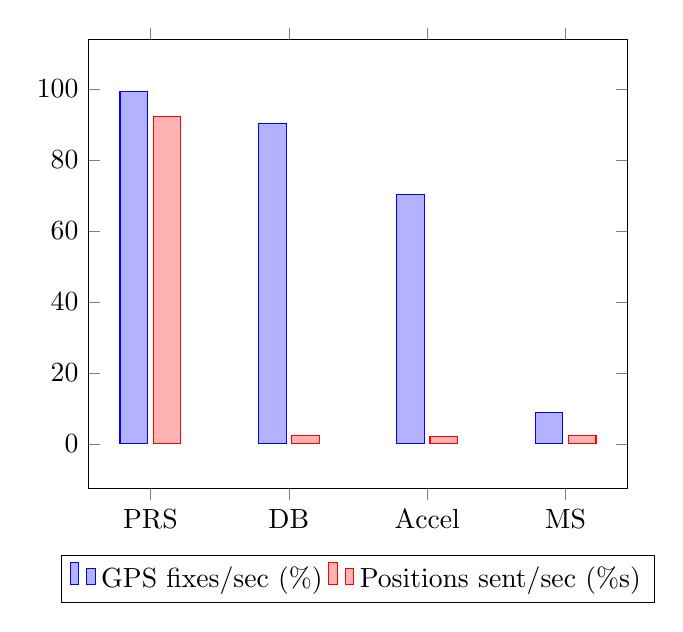
\begin{tikzpicture}
\begin{axis}
	[ybar,
	enlargelimits=0.15,
	legend style={at={(0.5,-0.15)},	anchor=north,legend columns=-1},
	symbolic x coords={PRS, DB, Accel, MS},
	xtick=data]
	
\addplot coordinates
	{(PRS,99.25) (DB,90.28) (Accel,70.15) (MS,8.92)};
\addplot coordinates
	{(PRS,92.22) (DB,2.31) (Accel,2.12) (MS,2.46)};

\legend{GPS fixes/sec (\%), Positions sent/sec (\%s)}
\end{axis}
\end{tikzpicture}
\caption{The amount of fixes read and the amount of positions sent to the server relative to time.}
\label{fixesandsendrelativetotime}
\end{figure}